\documentclass{article}
\usepackage[utf8]{inputenc}
\usepackage{graphicx}
\usepackage{booktabs}
\usepackage[binary-units]{siunitx}
\usepackage[running]{lineno}
\usepackage{setspace}
\usepackage[]{authblk} % options: affil-it
\usepackage{natbib}
\usepackage{amsmath}
\usepackage{amssymb}
\usepackage{bm}
\usepackage{hyperref}
\usepackage{subcaption}
\usepackage{mathtools}

\title{A two-stage parameter-fitting method for modeling truncated stem diameter distributions}

\author{}
\date{}

%\author{Gregory Paradis \thanks{Corresponding authour. Contact telephone number (418) 456-2208.}}
%\affil{\footnotesize Département des sciences du bois et de la forêt, Faculté de foresterie, de géographie et de géomatique, Pavillon Abitibi–Price, Université Laval, Québec, QC G1K 7P4, Canada. \texttt{gregory.paradis.1@ulaval.ca}}

%\author{Luc LeBel}
%\affil{\footnotesize Département des sciences du bois et de la forêt, Faculté de foresterie, de géographie et de géomatique, Pavillon Abitibi–Price, Université Laval, Québec, QC G1K 7P4, Canada. \texttt{luc.lebel@sbf.ulaval.ca}}

\begin{document}
\maketitle

%\clearpage
\begin{abstract}
  Statistical models predicting stem diameter distributions have found many applications in forestry.
  Stem diameter data collected from forest inventory sample plots may be both left- and right-truncated (i.e., non-merchantable stems below a certain size are not tallied, and maximum stem size is limited by ecological and other factors).
  The recommended procedure in this case is to fit the truncated data to special truncated forms of the target statistical distributions.
  Following this recommended procedure in practice can be technically challenging, and analysts may resort to fitting truncated data to complete distributions (yielding poor, biased fit in smaller size classes), or limiting analysis to target distributions that happen to have truncated forms available in the chosen software environment.
  We describe a new two-stage method for modelling stem diameter distributions from truncated datasets, using the complete form of any target distribution.
  We compare performance of our two-stage method to performance standard procedures (using a large truncated stem diameter dataset from Quebec, Canada), and show that our method essentially yields the same result as the best-practice truncated-distribution procedure.
\end{abstract}

%\linenumbers 
%\doublespace 

\clearpage
\section{Introduction}
\label{sec:introduction}

Stem diameters in forest stands are commonly characterized using common statistical distributions \citep{bailey1973quantifying, hyink1983generalized}, using best-fit parameters derived from plot data.
Collecting plot data is expensive, and in practice  the data used to fit diameter distributions will typically have been collected in a previous inventory sampling effort.
Thus, available plot data may have certain features that are not ideal for diameter distribution fitting.

If diameter is measured for all stems in each plot, the dataset can be described as \emph{complete}---this is the best-case scenario.
Sample lots in forest stands often contain many small stems, and measuring diameter of these small stems may be impractical or exceedingly expensive.
To improve efficiency of data collection, stems smaller than a known merchantability diameter threshold may not have been tallied---this results in a \emph{left truncated} dataset.
Furthermore, tree stems never grow to \emph{infinitely} large diameters---foresters will generally know the maximum expected stem diameter of a given species on a given site (i.e., stem diameter datasets are \emph{right truncated} at some known maximum diameter).
So, stem diameter plot data will generally be binned into a contiguous finite set of fixed-width diameter size classes, and can be described as \emph{doubly truncated}.

Complete forms of target statistical distributions are generally defined for domain $(0, \inf)$. 
Fitting doubly-truncated data to complete distributions on the interval $(0, \inf)$ using maximum-likelihood methods will generally result in poor fit and positively-biased sum of residuals.
The best-practice method fits truncated forms of target distributions to truncated data \citep{zutter1986characterizing}.
If the software environment used to perform best-fit parameter estimation does not already include truncated forms of target distributions, the analyst can attempt to implement one of the truncated forms published in the literature \citep{mittal1989estimating, hannon1999estimation, hegde1989estimation, ahmad2001moments, wingo1989left} or derive new doubly truncated forms using calculus---this involves solving the integral $F(x; \bm{P}) = \int_0^x f(t) dt$, which may be difficult or impossible for some distributions.
In practice, analysts working in non-academic settings may also have limited access to scientific literature, or may struggle with some of the coding or applied mathematical aspects of implementing new truncated distributions in their chosen software environment.

This paper describes a two-stage method we developed for fitting truncated data to \emph{complete} target distributions, which avoids overfitting the tails while still providing reasonable error bounds on best-fit parameters.
The method was originally developed to characterize stem diameter distributions in forest stands, but can be applied to any truncated dataset.

We present results from a computational experiment, where we compare performance of our two-stage complete (2sc) distribution method to one-stage complete (1sc) and one-stage truncated (1st) distribution methods.
We fit real stem diameter data (from permanent sample plots in Quebec, Canada) to Weilbull and gamma distributions, and show that our 2sc method is both simpler to implement and yields better fit results than 1sc and 1st methods.

  \section{Methods}
  \label{sec:methods}

  \subsection{Theoretical Background}
  \label{sec:methods_background}
  
  We use a weighted non-linear least squares (NLLS) algorithm to fit target distributions to truncated inventory data binned into diameter size classes of uniform width $W$.
  The objective function value of the NLLS problem minimizes the sum of squares of the residual terms
\begin{equation}
Z = \text{min} \quad \sum_{i \in I} e_i^2
\end{equation}
    with
  \begin{equation}
    e_i := e\left(f(x_i; \bm{P}), \hat{y}_i\right) = w_i \left[f(x_i; \bm{P}) - \hat{y}_i\right] 
  \end{equation}
  
  % \begin{equation}
  %   Z\left(f(x; \bm{\hat{P}})\right) = \text{min} \quad \sum_{\mathclap{i \in \{I|\hat{y}_i > 0\}}} e\left(f(x_i; \bm{P}), \hat{y}_i\right)^2 \label{eq:z}
  % \end{equation}
  % with
  % \begin{equation}
  %   e\left(f(x_i; \bm{P}), \hat{y}_i\right) = w_i \left[f(x_i; \bm{P}) - \hat{y}_i\right] 
  % \end{equation}
  where $x_i$ is the diameter corresponding to the center of bin $i \in I$, $f(x_i; \bm{P})$ is the value of the probability distribution function (PDF) at $x_i \in \bm{X}$ (given a vector of parameters $\bm{P}$). $\hat{y}_i \in \bm{\hat{Y}}$ represents the estimated stem density in bin $i$, which corresponds to the average of plot-wise stem density measurements (i.e., observed data).
  
  Note that residual terms are scaled by a weight factor $w_i = 1 - \text{min}(E_{\hat{y}_i}\hat{y}_i^{-1}, 1)$, which dampens the impact of $\hat{y}_i$ on $Z$ as a function of the relative margin of error $E_{\hat{y}_i}\hat{y}_i^{-1}$. We cap relative margin of error at 1 (negative values of $w_i$ would have the effect of \emph{rewarding} large residual value $f(x_i; \bm{P}) - \hat{y}_i$, which would make NLLS algorithm results unnecessarily difficult to interpret).  
  Thus, $w_i$ converges to 1 as relative margin of error approaches 0, and $w_i = 0$ if $E_{\hat{y}_i}\hat{y}_i^{-1} \geq 1$. 
  Note that if sampling error is high enough for all bins (due to insufficient sample size), such that  $w_i = 0, \forall i \in I$, the objective function value is 0 regardless of values of input data vector $\bm{\hat{Y}}$ and the NLLS optimisation problem becomes meaningless.

  The margin of error corresponds to the product $t\sigma_{\hat{y}_i}$ of the critical $t$ value (with $\alpha=0.05$ and $|\bm{\hat{Y}}|  - 1$ degrees of freedom) and bin-wise sampling error
  \begin{equation}
    \sigma_{\hat{y}_i}  = \sqrt{\frac{\sum_{j \in J} \left(y_{ij} - \hat{y}_i\right)^2}{|\bm{\hat{Y}}| - 1}}
  \end{equation}
  where $y_{ij}$ corresponds to the observed stem density in bin $i$ in sample plot $j$ \citep{schreuder2004statistical}.

  We normalize our binned data, such that $\sum_{i \in I} W\hat{y}_i = 1$.
  The domain of input data is bounded, such that $a \leq x_1 - W/2$ and $x_{|I|} + W/2 \leq b$, where $a > 0$ (i.e., we have a \emph{doubly truncated} dataset).
  Our dataset includes only merchantable stems with DBH larger than 9 cm (i.e., $a=9$), and contains no stems of with DBH larger than 61 cm (i.e.~$b = 61$).
  
The integral of the standard forms of the PDFs described above over the interval $[0, \infty)$ is 1 for any given vector of input parameters $\bm{P}$, that is
\begin{equation}
\int_0^\infty f(x; \bm{P}) dx =  1.
\end{equation}

Fitting the standard forms of $f$ to our truncated normalized binned data will generally produce poor fits, as the sum of residuals will be positively biased due to bounded domain (i.e.~$\sum_{i \in I} e_i>1$), with quality of fit inversely proportional to $b - a$.
The recommended procedure in this case is to fit the truncated data to a truncated form $f^T$ of the target distribution

\begin{equation}
    f^T(x; \bm{P}) = 
    \begin{cases}
     c f(x; \bm{P}), & a \leq x \leq b\\
      0, & \text{otherwise},\\
    \end{cases}
\end{equation}
where the scaling coefficient $c = \left[ \int_a^b f(x; \bm{P}) dx \right]^{-1}$ is the inverse of the integral of $f$ over the interval $[a, b]$, which ensures that the truncated distribution integrates to 1 (i.e.,  $\int_0^\infty f(x; \bm{P}) dx =  \int_a^b f(x; \bm{P}) dx =  1$). 
If the cumulative distribution function $F(x; \bm{P})$ is available, then we can define the scaling coefficient as $c = \left[ F(b; \bm{P}) - F(a; \bm{P}) \right]^{-1}$.
If no closed form of $F$ has been published (due to difficulty of algebraically solving the integral $F(x; \bm{P}) = \int_0^x f(t) dt$), then the value of scaling factor $c$ can only best estimated through numerical integration of $f$ (which is usually possible, but not always trivial to implement, depending on the shape of the function and programming skills of the analyst).
Parameter fitting for truncated datasets has received considerable attention in the literature, and truncted forms of many common distributions have been published \citep{mittal1989estimating, hannon1999estimation, hegde1989estimation, ahmad2001moments}, however correctly reproducing these methodologies in a practical setting can quickly become very complex (as each new target distribution to be tested requires a new truncated form to be derived and implemented in a form that is compatible with the software environment used for analysis).

In an effort to mitigate some of aforementionned challenges, we developed an alternative method for fitting truncated data to complete distributions.
The basis of our method is an observation that we can approximate the fit of $f_T$ using an augmented PDF $f'(x; \bm{P'}) = sf(x; \bm{P})$.
The global scaling parameter $s$ effectively relaxes the unity constraint on the integral of $f'$.
Thus, using $f'$, we obtain similar quality fits for any scaling of bin value vector $\bm{\hat{Y}}$, and match any shape that $f^T$ can take (on the interval $[a, b)$).

The variance $\sigma^2_{\hat{p}_j}$ of best-fit parameter estimator $\hat{p}_j \in \bm{\hat{P}}$ corresponds to element $j$ of the diagonal of the covariance matrix.
The covariance matrix, which is automatically calculated by most software implementations of the NLLS algorithm, corresponds to the inverse of the  negative of the expected values of the Hessian matrix $-E[H(\bm{\hat{P}})]$, where the Hessian $H(\bm{\hat{P}})$ is the matrix of second derivatives of the likelihood function $\mathcal{L}$ with respect to $\bm{\hat{P}}$.
Standard error $\sigma_{\hat{p}_j} = \sqrt{\sigma^2_{\hat{p}_j}}$ of parameter $\hat{p}_{j} \in \bm{\hat{P}}$ corresponds to the square root of the variance.

Note that variance estimates are only correct asymptotically.
In practice, fitting algorithms will use numerical approximations of Hessian matrix values.
Quality of finite approximations of the second derivatives of $\mathcal{L}$ will tend to be proportional to sample size $|\bm{\hat{Y}}|$, inversely proportional to distance from parameter constraint boundaries, and inversely proportional to the number of parameters $|\bm{\hat{P}}|$.
Thus, augmenting $f$ with global scaling parameter $s$ will have a negative effect on the quality of parameter estimation error bounds. 

Parameter estimation error bounds for augmented function  $f'(x; \bm{P'})$ can be improved, without deteriorating fit quality, by solving the fitting problem in two stages.
In the first stage, we determine $\bm{\hat{P'}}$ by solving for $Z(f'(x; \bm{\hat{P'}}))$.
For the best-case scenario, where $f'(x; \bm{P'})$ is fitted to an infinitely large sample $\bm{\hat{Y}}$ randomly drawn from $f'(x; \bm{\hat{P'}})$, the estimated value of scaling parameter $\hat{s} \in \bm{\hat{P'}}$ will completely eliminate the bias in the sum of residuals $\sum_{i \in I} e(f(x_i; \bm{\hat{P}}), \hat{y}_i)$, such that $\int_a^b f(x; \bm{\bar{P'}}) dx = \sum_{i \in I} W\hat{y}_i$.

In the second stage, we solve for  $Z(f''(x; \bm{\hat{P}}, \hat{s}))$, where $f''$ corresponds to our augmented distribution $f'$ with the scaling parameter value fixed at $s = \hat{s}$ (i.e.~only the original vector of parameters $\bm{P}$ is optimized by the fitting algorithm).

The shape distributions from both stages are equivalent, such that
\begin{equation}
 Z(f'(x; \bm{\hat{P'}})) \simeq Z(f''(x; \bm{\hat{P}}, \hat{s})). 
\end{equation}

However, error vector $\bm{\sigma}_{\hat{P}}$ and parameter covariance (which can be estimated from off-diagonal elements of the covariance matrix) estimated in the second stage will tend to be more reliable.


\subsection{Computational Experiment}
\label{sec:methods_experiment}

We ran a computational experiment on real plot sample data, comparing the performance of our two-stage method to the recommended one-stage truncated distribution method.

The test stem diameter dataset is compiled from a database of over 1 million stems from permanent sample plot data collected in Quebec, Canada. We filtered this dataset to include only plots in fully stocked, undisturbed, mature stands, that were measured using a similar data collection protocol. We aggregated the filtered plots into 30 meta-plots, based on species composition and cover types.
Data from each meta-plot was binned into 26 bins representing 2 cm wide diameter size classes (i.e., $W=2$)---these datasets are doubly truncated ($a=9$, $b=61$).

We ran our experiment on 3 of the 30 metaplots (representing 3 species groups and 3 cover types), to test performance of our 2sc method across a wide range of forest types---the meta-plots correspond to spruce-pine-fir-larch (SPFL) in softwood stands (i.e., SPFL-S), white birch in mixedwood stands (i.e., birch-M), and sugar maple in hardwood stands (i.e., maple-H).

Data from each meta-plot was fit to both two-parameter Weibull and two-parametr gamma distributions, which have been used to characterize stem diameters in forest stands \citep{bailey1973quantifying, cao2004predicting, ducey2015sizebiased, zutter1986characterizing, hafley1977statistical}.
Both Weibull $f_W(x;a, b)$ and gamma $f_G(b, p)$ distributions are special cases of the three-parameter generalized gamma distribution $f_{GG}(x; a, b, p)$ (i.e., fixing either $p=1$ or $a=1$).

The PDF $f_{GG}$ of the generalized gamma distribution has the following form

\begin{equation}
f_{GG}(x; a, \beta, p) = \frac{ax^{ap-1}e^{-\left(\frac{x}{\beta}\right)^a}}{\beta^{ap}\Gamma(p)}, \qquad a > 0, \beta > 0, q > 0
\end{equation}
defined for $x > 0$, where $\Gamma(p)$ represents the gamma function (not to be confounded with the gamma, or generalized gamma, distributions), which is given by
\begin{equation}
\Gamma(p) = \int_0^\infty x^{p-1}e^{-x} dx.
\end{equation}

Our software framework for this experiment implements the $f_{GG}$ and fixes the appropriate parameters to induce $f_W$ and $f_G$. 
We approximated the truncated form of $f^T_{GG}$ of the complete generalized gamma distribution using an approximated CDF $F_{GG}$, which we compiled using a numerical integration procedure.
The numerical integration approach likely introduces some error (relative to algebraic integration), but has the notable advantage of working as-is with \emph{any} arbitrary PDF $f$.
This approach avoids reliance on availability of a closed-form arithmetic formulation of $F$, which may require some complex calculus to derive $F(x; \bm{P}) = \int_0^\infty f(x; \bm{P}) dx $.  

Our test data is binned into 26 size classes (i.e.., $n = 26$), and the distributions we are fitting have between 2 and 4 parameters (i.e., $3 \leq K \leq 5$).
\citet{burnham2002model} recommend using the small-sample form of the Akaike information criterion (AICc) when $n/K < 40$.
We use AICc to evaluate goodness-of-fit for each combination of meta-plot, target distribution, and fit method.
AICc is given by
\begin{equation}
\text{AICc} = AIC + \frac{2K(K + 1)}{n - K - 1}
\end{equation}
with
\begin{equation}
\text{AIC} = 2K - n\ln\left(\frac{\chi^2}{n}\right)
\end{equation}
where $K=|\mathbf{P}|+ |\mathbf{Q}|+1$  (i.e., sum of cardinalities parameter vectors $\mathbf{P}$ and  $\mathbf{Q}$ the  plus one for the $\mu$ parameter of the implicit i.i.d. Gaussian error distribution of input data vector $\mathbf{\hat{Y}}$), $n=|\mathbf{\hat{Y}}|$ (as recommended in \citealp{burnham2002model}), and $\chi^2$ is the sum of squared residuals given by
\begin{equation}
\chi^2 = \sum_{i \in I} e\left(f(x_i; \bm{\hat{P}}), \hat{y}_i\right)^2
\end{equation}

We report estimated parameter values and standard error on parameter estimates, as well as
results of AICc, $\chi^2$, and Kolmogorov-Smirnov (KS) goodness-of-fit tests.
%For a given meta-plot and target distribution, $\Delta$AICc, $\Delta\chi^2$, and $\Delta$KS are calculated relative to the score of the best fit method.

Note that we count $a$, $b$ and $s$ extra parameters in our definition of $\mathbf{Q}$ for computation of AICc scores.
Thus we define parameter $K$ as 

\begin{align} K_{1sc} & =  |\mathbf{P}| + |\{\}| + 1 = |\mathbf{P}| + 1,\\
  K_{1st} & =  |\mathbf{P}| + |\left{a, b\right}| + 1 = |\mathbf{P}| + 3,\\
  K_{2sc} & = |\mathbf{P}| + |\left{s\right}| + 1 = |\mathbf{P}| + 2
  \end{align}

  for 1sc, 1st, and 2sc fit methods, respectively. 


  \section{Results}
  \label{sec:results}

  Figure \ref{fig:results} shows best-fit distributions plotted against empirical input data distribution, binned by diameter class.
  Subfigure rows correspond to meta-plots (i.e., SPFL in softwood stands, white birch in mixedwood stands, sugar maple in hardwood stands).
  Sufigure columns correspond to target distributions (i.e., Weibull, gamma).
  Each subfigure shows best-fit distributions for each of three fit methods (i.e., 1sc, 1st, 2sc).
  Fit method \emph{1sc} (shown with a solid line) is the one-stage method with complete distribution.
  Fit method \emph{1st} (shown with a dashed line) is the one-stage method with truncated distribution.
  Fit method \emph{2sc} (shown with a dotted line) is the two-stage method with complete distribution.
  
  Table \ref{tab:results} reports estimated parameter values, standard error on parameter estimates, and $\Delta$ AICc (indexed by meta-plot and fit method).

  \begin{figure}[h!]
    \centering
    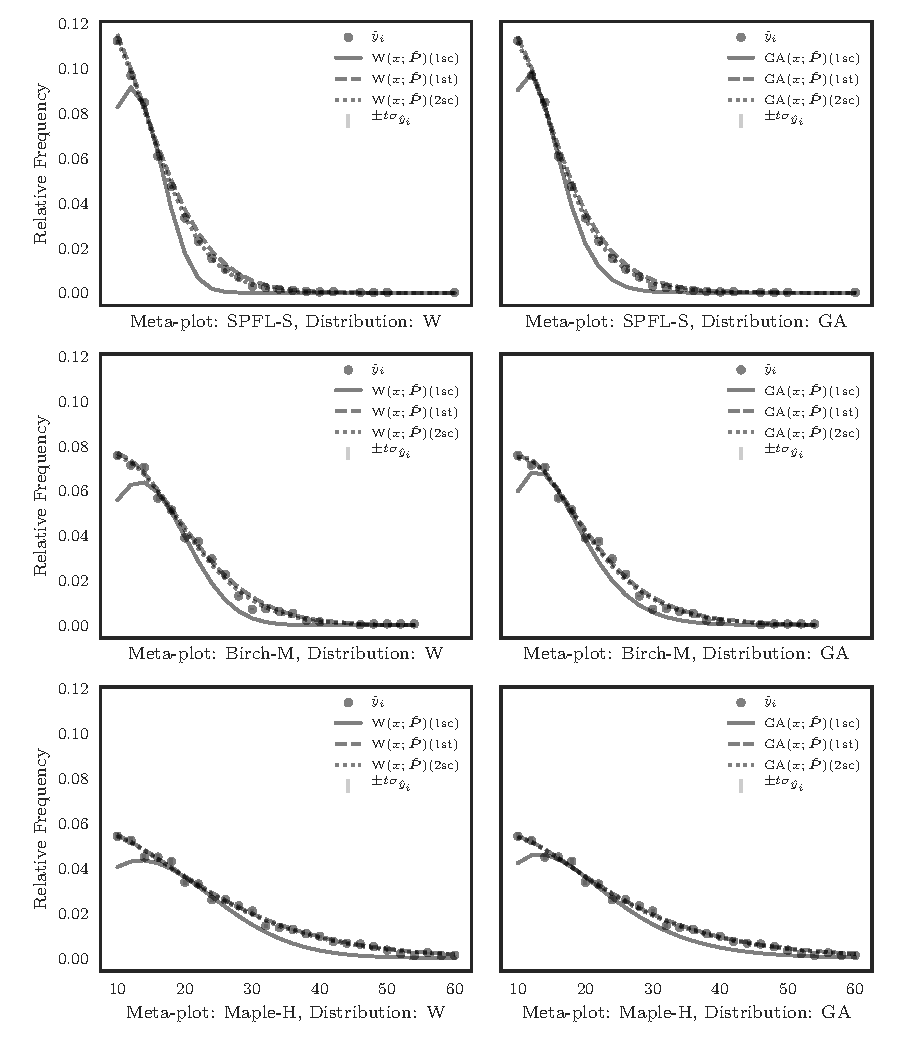
\includegraphics[width=1.0\textwidth]{images/results}
    \caption{Weibull and gamma best-fit distributions (subfigure columns) for three meta-plots (subfigure rows), plotted against empirical input data distribution. Empirical distributions (binned by 2 cm diameter class) are shown with gray circles with bin-wise sampling error shown with light gray error bars.  Each subfigure shows results of applying the three fit methods (1sc, 1st, 2sc) to meta-plot data from a different combination of species group and cover type.}
  \label{fig:results}
\end{figure}


\begin{table}[h!]
  {\footnotesize
\begin{tabular}{lllllr}
\toprule
Species & Cover & Dist.   & Fit  & Parameters & $\Delta$AICc \\
Group   & Type  & Name  & Method & & \\
\midrule

SPFL & S & W & 1sc & a = 3.20$\pm$0.25 & 88 \\
 &  &  &  & $\beta$ = 13.58$\pm$0.43 &  \\
 &  &  & 1st & a = 1.64$\pm$0.07 & 30 \\
 &  &  &  & $\beta$ = 11.96$\pm$0.32 &  \\
 &  &  & 2sc & a = 1.77$\pm$0.01 & \textbf{0} \\
 &  &  &  & $\beta$ = 12.04$\pm$0.07 & \textbf{} \\
 &  & GA & 1sc & $\beta$ = 1.40$\pm$0.15 & 76 \\
 &  &  &  & p = 9.28$\pm$0.99 &  \\
 &  &  & 1st & $\beta$ = 3.54$\pm$0.23 & 27 \\
 &  &  &  & p = 3.42$\pm$0.28 &  \\
 &  &  & 2sc & $\beta$ = 3.09$\pm$0.04 & \textbf{0} \\
 &  &  &  & p = 3.92$\pm$0.05 & \textbf{} \\
Birch & M & W & 1sc & a = 2.58$\pm$0.18 & 52 \\
 &  &  &  & $\beta$ = 16.18$\pm$0.55 &  \\
 &  &  & 1st & a = 1.71$\pm$0.07 & 6 \\
 &  &  &  & $\beta$ = 15.63$\pm$0.28 &  \\
 &  &  & 2sc & a = 1.77$\pm$0.03 & \textbf{0} \\
 &  &  &  & $\beta$ = 15.52$\pm$0.21 & \textbf{} \\
 &  & GA & 1sc & $\beta$ = 2.56$\pm$0.25 & 39 \\
 &  &  &  & p = 6.00$\pm$0.60 &  \\
 &  &  & 1st & $\beta$ = 4.65$\pm$0.32 & 3 \\
 &  &  &  & p = 3.28$\pm$0.25 &  \\
 &  &  & 2sc & $\beta$ = 4.42$\pm$0.14 & \textbf{0} \\
 &  &  &  & p = 3.43$\pm$0.11 & \textbf{} \\
Maple & H & W & 1sc & a = 1.96$\pm$0.12 & 66 \\
 &  &  &  & $\beta$ = 19.46$\pm$0.77 &  \\
 &  &  & 1st & a = 1.32$\pm$0.05 & 4 \\
 &  &  &  & $\beta$ = 19.30$\pm$0.33 &  \\
 &  &  & 2sc & a = 1.35$\pm$0.02 & \textbf{0} \\
 &  &  &  & $\beta$ = 19.10$\pm$0.30 & \textbf{} \\
 &  & GA & 1sc & $\beta$ = 5.27$\pm$0.49 & 55 \\
 &  &  &  & p = 3.51$\pm$0.33 &  \\
 &  &  & 1st & $\beta$ = 10.45$\pm$0.67 & 3 \\
 &  &  &  & p = 1.81$\pm$0.13 &  \\
 &  &  & 2sc & $\beta$ = 10.01$\pm$0.27 & \textbf{0} \\
 &  &  &  & p = 1.87$\pm$0.05 & \textbf{} \\
  
  \bottomrule
  \end{tabular}
}
  
\caption{For each of three fit methods (1sc, 1st, 2sc), we report estimated parameter values, standard error on parameter estimates, and $\Delta$AICc for for best-fit parameters on each of three combonation of species group and cover type (SPFL-S, Birch-M, Maple-H) and two target distributions (W, GA).}
\label{tab:results}
\end{table}

$Delta$AICc results in Table \ref{tab:results} show that relative ranking of the three methods is consistent across all six meta-plot--distribution combinations---method 2sc is the best, with method 1st yielding very similar (but slightly inferior) results, and method 1sc having the highest (worst) scores.

These observations can be confirmed through visual inspection of the goodness of fit in Figure \ref{fig:results}.
Best-fit curves from method 1sc (solid lines) tend to be shifted downward relative to the data, have poor fit on the far left and in the middle of the data range.
Best-fit curves from methods 1st and 2sc are almost perfectly coincident, with 2sc curves fitting the data slightly better than the 1st curves.
 
  
 %\section{Discussion}
  %\label{sec:discussion}

  \section{Conclusion}
  \label{sec:conclusion}

  When fitting statistical distributions to truncated data, the literature recommends using the 1st fit method (i.e., fitting the truncated dataset to a truncated distribution), rather than the more niaive 1sc method (i.e., fitting the truncated dataset to a complete distribution)---the rationale here is that using the 1st fit method mitigates problems with bias and poor fit inherent to the 1sc method.
  Results from the computational experiment presented in \S\ref{sec:results} confirm that the 1st method does indeed yield consistently better fits than the 1sc method.

  However, implementation the 1st method in practice can be technically challenging, as it requires the analyst to derive mathematical formulations and software implementations of truncated forms of all target distributions that are to be fit to the truncated dataset. This generally involves numerical integration of the PDF of the complete distribution, (or having access to the CDF of the complete distribution), as well as some non-trivial programming tasks to implement the truncated PDF forms in the software environment used for analysis.
  For some more novice analysts, one or more of these challenges may be problematic.

  In this paper we presented a new two-stage fit method (2sc), which combines the strong points of both other methods (i.e., slightly out-performs 1st, no harder to implement in practice than 1sc).
  There are no obvious down-sides to 2sc, therefore we recommend that this be the new recommended method for practical applications.

  Consistently with the principles of FAIR\footnote{Findable, Accessible, Interoperable, Reusable.} science \citep{stall2019make, wilkinson2016fair}, we implemented our experiment in a Jupyter Notebook using open-source Python libraries, which is available for download from a public GitHub repository\footnote{https://github.com/gparadis/foo}.  The repository includes a complete anonymized sample dataset, which can be used to replicate all results presented here.
  
\section{Acknowledgements}

This study was supported by funding from the \emph{FORAC Research Consortium}, as well as \emph{Genome BC} and \emph{Genome Quebec}.

\begin{nolinenumbers}
\bibliographystyle{apalike}
%\nocite{*} % adds all references in the bib file to the bibliography (cited or not)
\bibliography{refs.bib}
\end{nolinenumbers}


\end{document}


%%% Local Variables:
%%% mode: latex
%%% TeX-master: t
%%% End:
